\documentclass[reqno,10pt]{amsart}
\usepackage[colorlinks = true, linkcolor=blue,
            urlcolor=red,
            citecolor=olive]{hyperref}
\usepackage[utf8]{inputenc}
\usepackage[T1]{fontenc}
\usepackage{amsmath}
\usepackage{tikz}
\usepackage{tikz-3dplot}
\usepackage{amssymb}
\usepackage[colorinlistoftodos]{todonotes}
\tikzset{surface/.style={draw=blue!70!black, fill=blue!40!white, fill opacity=.6}}
\tikzset{circ/.style={shape=circle, inner sep=1.5pt, draw, node contents=}}

\newcommand{\type}{\tau}

\newcommand{\Sph}{\mathbb{S}}

\begin{document}

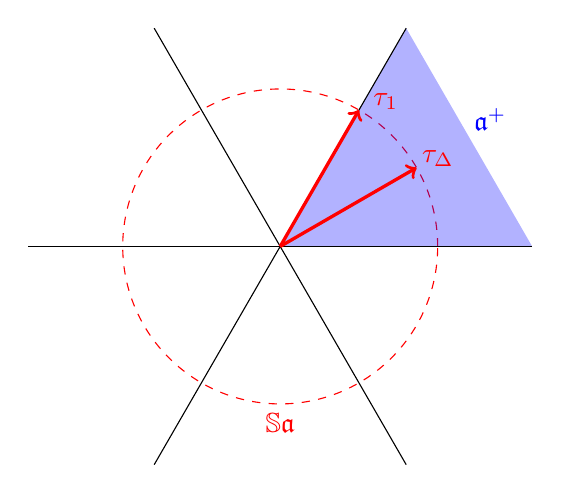
\begin{tikzpicture}[scale=2]
\draw[red, thin, dashed] (0,0) circle(1);
\fill[blue, opacity=.3] (0,0) -- (0:1.6) -- (60:1.6);
\draw (0,0) -- (0:1.6);
\draw (0,0) -- (60:1.6);
\draw (0,0) -- (120:1.6);
\draw (0,0) -- (180:1.6);
\draw (0,0) -- (240:1.6);
\draw (0,0) -- (300:1.6);
\draw[->,very thick, red] (0,0) -- (30:1);
\node[above right,red] () at (28:.95) {$\type_\Delta$};
\draw[->,very thick, red] (0,0) -- (60:1);
\node[right,red] () at (60:1.06) {$\type_1$};
\node[above right,blue] () at (30:1.35) {$\mathfrak{a}^+$};
\node[below,red] () at (270:1) {$\Sph\mathfrak{a}$};
\end{tikzpicture}

\end{document}